\renewcommand{\appref}[1]{, c.f. Appendix, Def.\,\ref{#1}}
 
%As was have seen, \Chainmail assertions not only talk about the contents of the current state (stack frame and heap),
%but they also talk about future and past states, Therefore, 
The meaning of \Chainmail assertions is parametric with an
underlying object-oriented programming language, with modules  as repositories of code, classes with fields, methods and
ghostfields, objects described by classes, a way to link  modules into larger ones, and a concept of 
program execution\footnote{We believe that \Chainmail can be applied to 
any language with these features.}.

We have developed   \LangOO, a \jm{deterministic and} minimal such object-oriented language, which we
outline in  this section. 
We  describe the novel aspects of \LangOO, and 
summarise the more conventional parts, relegating  full, and mostly unsurprising,
definitions %for  \LangOO~appear 
to Appendix \ref{app:LangOO}.
 

Modules are central to \LangOO, as they are to \Chainmail. As modules are repositories
of code, we adopt the common formalisation of modules as maps from 
class identifiers to class definitions\appref{defONE}. We use the terms module and component in an
analogous manner to class and object respectively.  \LangOO is untyped 
\sophia{for several reasons. Many popular programming languages are untyped.
The external module might be untyped, and so it is more
general to consider everything as untyped.
Finally, 
a solution that works for an untyped language %(doesnt depend on types) 
will also apply to a typed language, while the converse is not true.
}
%, where we link with external modules which come without any
%guarantees.

 Class definitions consist of field, method and ghost field declarations\appref{def:syntax:classes}.
Method bodies are sequences of 
statements, which  can be field reads or field assignments, object
creation, method calls, and return statements. 
%All else, \eg booleans, conditionals, loops,  can be encoded.
Fields are private in the sense of C++ or Java: they can only be read or
written by methods of the current class.
This is enforced by the operational semantics, \cf Fig.~\ref{fig:Execution}.
We  discuss ghost fields in the next section.

Runtime configurations, $\sigma$,  contain   all the usual information about execution snapshots: the heap, and a
stack of frames. 
% sd dropped fillowing sentence as it appears afterwards
%The code to be executed is kept as part of the runtime configuration:
%
Each frame consists of a continuation, \prg{contn}, describing the remaining code to be executed by the
frame, and a map from
variables to values. Values are either addresses or sets of addresses; sets 
are needed to deal with assertions which quantify over sets of
objects, such as assertions
(1) and (2) from section \ref{sect:motivate:Bank}.
% 
We define \emph{one-module} execution  through a judgment of the form $\M, \sigma \leadsto \sigma'$ in Appendix~\ref{app:LangOO}, Fig.~\ref{fig:Execution}. 
%
  
\subsection{Connectivity}
Many programs are only allowed to pass on objects under certain conditions. This is to keep these objects safe from code that shouldn't have access to them, such as malicious external modules, or even other internal objects that were not expecting them, and whose actions may have unintended consequences. \mrr{As shown in assertion (3) in section~\ref{sect:motivate:Bank}, in} \Chainmail restricting access is expressible: assertions can ensure that objects which will need access have a means to gain it. Alternatively, they can ensure that when an object's state changes, some other object could have had access to cause that change.

However, to prove these assertions, it is necessary to ensure code only has access to objects it is directly passed. This allows us to check only connections created explicitly to check these assertions. To check code only has access to what it is passed, we can ensure any method call---the barrier between \Mrr{the private state of different objects}---only \emph{connects} to what its parameters \Mrr{can obtain} access to. This can be expressed formally as:

\begin{lemma}[Method call connectivity]
\label{lemma:method_call_connectivity}
\begin{align*}
\forall M . \forall \sigma, \sigma'. &\forall \alpha, \alpha' \in \chi. [\\
&\sigma\text{.cont} = \x_0.\m(\x_1,\dots\x_n) \wedge \M,\sigma\leadsto^\text{call} \sigma' \wedge \text{access}_{\sigma'}\langle \alpha,\alpha'\rangle 
\longrightarrow\\
&\text{access}_\sigma\langle\alpha,\alpha'\rangle
\\&\quad \vee\Mrrz{
\exists \alpha'' \alpha'''. (\exists k. (\x_k = \alpha'') \wedge \exists k. (\x_k = \alpha''') \wedge 
\text{access}^*_\sigma\langle \alpha'',\alpha\rangle \wedge 
\text{access}^*_\sigma\langle \alpha''',\alpha'\rangle)}\\
&]
\end{align*}
\end{lemma}

This states that for any method call, if two objects are connected in the configuration when the call has completed, then either they were originally connected, or an object explicitly passed to the call could \Mrr{obtain access} to both. \mrr[Should we mention how \Chainmail doesn't need this guarantee]{This holds due to the lack of ambient authority in \LangOO, preventing methods from implicitly expanding their connectivity}.


\mrr{An example of where the lemma is useful is for assertion (3) in the Bank example, as given in section~\ref{sect:motivate:Bank}. Here, the assertion states if someone external will have access to an account, then someone external must have had access to it originally. Lemma~\ref{lemma:method_call_connectivity} renders it sufficient to check the values passed at the boundaries---method calls, parameters, and returns---to prove that a given program doesn't leak information. By checking the methods of the \prg{Account} and \prg{Bank} classes, we need only ensure they do not pass out account references through \prg{return}s or method calls to external objects. From an internal method, an external call can only access the objects it is given, so if there is no \prg{Account} passed it will be unable to access one. From an external method, an internal call will either pass an \prg{Account} at a boundary by providing or returning the \prg{Account} reference, or, as per the disjunction in lemma~\ref{lemma:method_call_connectivity}, the external object must have originally had access before the the internal code began executing. This final case must hold if the internal code doesn't pass an \prg{Account} reference, in which case there is no leak since the external object already held a reference to the \prg{Account}.  Whilst checking the boundaries may be the expected requirement for proving the validity of assertion (3), lemma~\ref{lemma:method_call_connectivity} is important to prove to ensure the soundness of this approach, as it proves any method is unable to expand its connectivity beyond that which it is given.
}

To evaluate the entire call, we define a new reduction operator, $\leadsto^\text{call}$, which executes function calls in one step. It does this by skipping any intermediate reduction steps with the additional frames for the method call and its child calls in the stack.

\begin{definition}[Call-as-step execution]
\label{def:call_execution} 
Given runtime configurations $\sigma$,  $\sigma'$,  and a module $\M$ we define call-as-step execution as follows:
 
\begin{itemize}
\item\Mrr[This definition has been updated]{
$\M, \sigma \leadsto^\text{call} \sigma'$ \IFF
there exist $n\geq 2$, runtime configurations $\sigma_1$ ... $\sigma_n$,
frames~$\phi$,~$\phi'$, and heaps~$\chi$,~$\chi'$, such that}
\begin{itemize}
\item
$\sigma = (\phi \cdot \psi, \chi)$, \ \ \ \ and\ \ \ \
$\sigma' = (\phi' \cdot \psi, \chi')$, for some stack $\psi$
\item
$\sigma_1=(\phi, \chi)$,\ \ \ \ \ \ \ \ and\ \ \ \ $\sigma_n=(\phi', \chi')$.
\item
$\M, \sigma_i \leadsto \sigma_{i+1}$,\ \ \ \ \ \ \ for $1\leq i \leq n\!-\!1$,
\item
 $\sigma_i = (\psi'\cdot\phi'', \_)$,\ \ \ \ for $2\leq i \leq n\!-\!1$, some frame $\phi''$, and some non-empty stack $\psi'$ 
\end{itemize}
\end{itemize}
\end{definition}

We define a connective $\text{access}\langle\_,\_\rangle$ similar to $\CanAccess{\_}{\_}$ in \Chainmail, to encode when two objects are connected. However, the receiver and parameters can gain access to any object they initially only have indirect access to. If one of their fields has access to an object, this object could be passed up, either directly if they are of the same class, or otherwise by a method invocation. This could happen to any depth, and so any $n^\text{th}$ child field must be considered. We therefore define a transitive access predicate, $\text{access}^*\langle\_,\_\rangle$, to encode this property.

\begin{definition}[\Mrrz{Access relations}]
\label{def:access_rel} \Mrr[Defintion now given]{Given runtime configuration $\sigma$, and addresses $\alpha$ and $\alpha'$, we define access and transitive access as:}

\begin{itemize}
\item $\text{access}_{\sigma}\langle\alpha,\alpha'\rangle \triangleq \alpha = \alpha' \vee \exists f. (\sigma(\alpha, \f) = \alpha') \vee \alpha = \interp{\prg{this}}{\sigma} \wedge \exists x. (\alpha' = \interp{\x}{\sigma})$
\item \Mrr[I have written up the formal definition for this, but left it out as it's obvious and takes up space]{$\text{access}^*_{\sigma}\langle\alpha,\alpha'\rangle$ is the transitive closure of $\text{access}_\sigma\langle\alpha,\alpha'\rangle$}
%\item $\text{access}^*_{\sigma}\langle\alpha,\alpha'\rangle \triangleq \exists k (\text{access}^k_\sigma\langle\alpha,\alpha'\rangle)$ \IFF $\text{access}^n_\sigma\langle\alpha, \alpha'\rangle$, $n \ge 1$ such that
%\begin{itemize}
%\item $\text{access}^n_\sigma\langle\alpha,\alpha'\rangle = \begin{cases}
%\text{access}_\sigma\langle\alpha,\alpha'\rangle & n = 1\\
%\exists\alpha''.(\text{access}_\sigma^{(n-1)}\langle\alpha,\alpha''\rangle \wedge \text{access}\langle\alpha'',\alpha'\rangle) & n \ge 1
%\end{cases}$
%\end{itemize}
\end{itemize}
\end{definition}

To prove lemma~\ref{lemma:method_call_connectivity}, we use a series of auxiliary lemmas. The first, lemma~\ref{lemma:local_variable_connectivity}, concerns local variables, and says \Mrr{under constrained reduction,} that if an object is referred to by a local variable in any frame, then the initial receiver, \prg{this}, was transitively connected to it.

\begin{lemma}[Local variable connectivity]
\label{lemma:local_variable_connectivity}
$$\forall M. \forall \sigma \forall \phi. \forall \psi.\forall \x. \forall \alpha \in \sigma. (M,\sigma \lceil\leadsto^*\rceil (\psi, \_) \wedge \phi \in \psi \wedge \interp{\x}{\phi} = \alpha \longrightarrow \text{access}^*_{\sigma}\langle \interp{\prg{this}}{\sigma}, \alpha\rangle)$$
\end{lemma}

The strengthening of this lemma to all frames of the stack, instead of simply the top frame, enables its inductive proof to handle the \prg{return} case. In this case we need to prove that the initial receiver can access the variables in the new top frame, which was previously the second top frame. Knowing \Mrr{the receiver can access local variables in all frames inductively renders this step} straightforward. \Mrr{We use constrained reduction to prevent the computation from returning from the initial method, which would render the initial receiver irrelevant.}

We then prove that if two objects are connected by the final configuration, either the initial \prg{this} had access to both, or they were initially connected.
\Mrr{
\begin{lemma}[Receiver connectivity]
\label{lemma:receiver_connectivity}
\begin{align*}
\forall M. \forall \sigma, \sigma' \forall \alpha, \alpha' \in \sigma. &\ (M,\sigma \lceil\leadsto^*\rceil \sigma' \wedge \text{access}_{\sigma'}\langle \alpha, \alpha'\rangle \longrightarrow\\
&\quad \text{access}^*_\sigma \langle \interp{\prg{this}}{\sigma}, \alpha\rangle \vee \text{access}_\sigma\langle{\alpha, \alpha'}\rangle)
\end{align*}
\end{lemma}
}

This follows intuitively from lemma~\ref{lemma:local_variable_connectivity}, since any connections made must occur through local variables by the grammar of \LangOO. From here we can prove the original lemma~\ref{lemma:method_call_connectivity} by noticing in the next step, the receiver will have access to the parameters, and so lemma~\ref{lemma:receiver_connectivity} applies.

\subsection{\sdf{Modules satisfying assertions}}

Finally, we define satisfaction of assertions by modules: a module
$\M$ satisfies an assertion $\A$ if for all other potential modules $\M'$, in all configurations arising from executions of $\M\mkpair\M'$, the assertion $\A$ holds.

\begin{definition}
\label{def:module_satisfies}
For any module $\M$, and  assertion $\A$, we define:
\begin{itemize}
\item
$\M \models \A \ \ \  \ \ \ \ \ \mbox{
if               } \ \ \  \ \ \  \  \forall \M'.\forall \sigma_0 \in \Initial{\M \mkpair \M'}.\forall\sigma\in\Arising{\M \mkpair  {\M'}, \sigma_0}. [\ \M \mkpair  {\M'}, \sigma_0 , \sigma \models \A\ ]$
\end{itemize}
\end{definition}
  
  

\subsection{\sdf{Linking and two-state execution}}

We define a module linking operator \  $\link$ \  so that
$\M\link\M'$ is the union of the two modules, provided that their domains are disjoint\appref{def:link}.
 %
As we said in section \ref{sect:overviewmodel}, we distinguish  between the internal and external module. \sophia{We consider execution  from the view of the
external module, and treat}  execution of 
methods from the internal module as atomic. For this, we define \emph{two-module execution}  based on
one-module execution as follows:

%Susan: I don't understand this when n = 2
\begin{definition}
\label{def:execution:internal:external}
\label{def:module_pair_execution} 
Given runtime configurations $\sigma$,  $\sigma'$,  and a module-pair $\M \mkpair \M'$ we define
execution where $\M$ is the internal, and $\M'$ is the external module as below:
 
\begin{itemize}
\item
$\M \mkpair \M', \sigma \leadsto \sigma'$ \IFF
there exist  $n\geq 2$ and runtime configurations $\sigma_1$,  ...
$\sigma_n$, \\such that
\begin{itemize}
\item
$\sigma$=$\sigma_1$,\ \  \ \ and\ \ \ \ $\sigma_n=\sigma'$.
\item
$\M \link \M', \sigma_i \leadsto \sigma_{i+1}$,\  \  for $1\leq i \leq n\!-\!1$
\item
$\ClassOf{\this} {\sigma}\not\in dom({\M})$,  \ \  \ \ and\ \ \ \
$\ClassOf{\this} {\sigma'} \not\in dom({\M})$,
\item
 $\ClassOf{\this} {\sigma_i} \in dom({\M})$,\ \ \ \ for $2\leq i \leq n\!-\!\Mrrz{1}$
\end{itemize}
\end{itemize}

\end{definition}
 
In the definition above,  $\ClassOf {\x} {\sigma} $ looks up the class of the object \sophia{stored} at \x\appref{def:interp}.
% If  $n$  has the value $2$, %. In this case the final bullet is trivial and  
%then  there exists a direct, external transition from $\sigma$ to $\sigma'$.  
 For example, for $\sigma_4$ as in Section \ref{sect:chainmail} whose next statement to be executed 
 is  $\prg{a}_2.\prg{deposit}{\prg{(}}\prg{a}_3,\prg{360}{\prg{)}}$,  we would have 
 a sequence of configurations $\sigma_{41}$, ... $\sigma_{4n}$,  $\sigma_{5}$ so that the
  one-module execution gives
 $\M_{BA2}, \sigma_4 \leadsto \sigma_{41} \leadsto \sigma_{42} ... \leadsto \sigma_{4n}   \leadsto \sigma_{5}$.
This would correspond to an atomic evaluation in the two-module execution: \  \
 $\M_{BA2}\mkpair \M', \sigma_4 \ \leadsto \sigma_5$ (see Fig.\ref{fig:VisibleStates}; \sophia{where blue stands for $\sigma(this)\!\in\!M_1$,%
   and  orange for $\sigma(this)\!\in\!M_2$}).


\begin{figure}[htb]
  \vspace*{-2.5mm}
  \begin{center}
   \begin{minipage}{0.80\textwidth}
     \begin{center}
       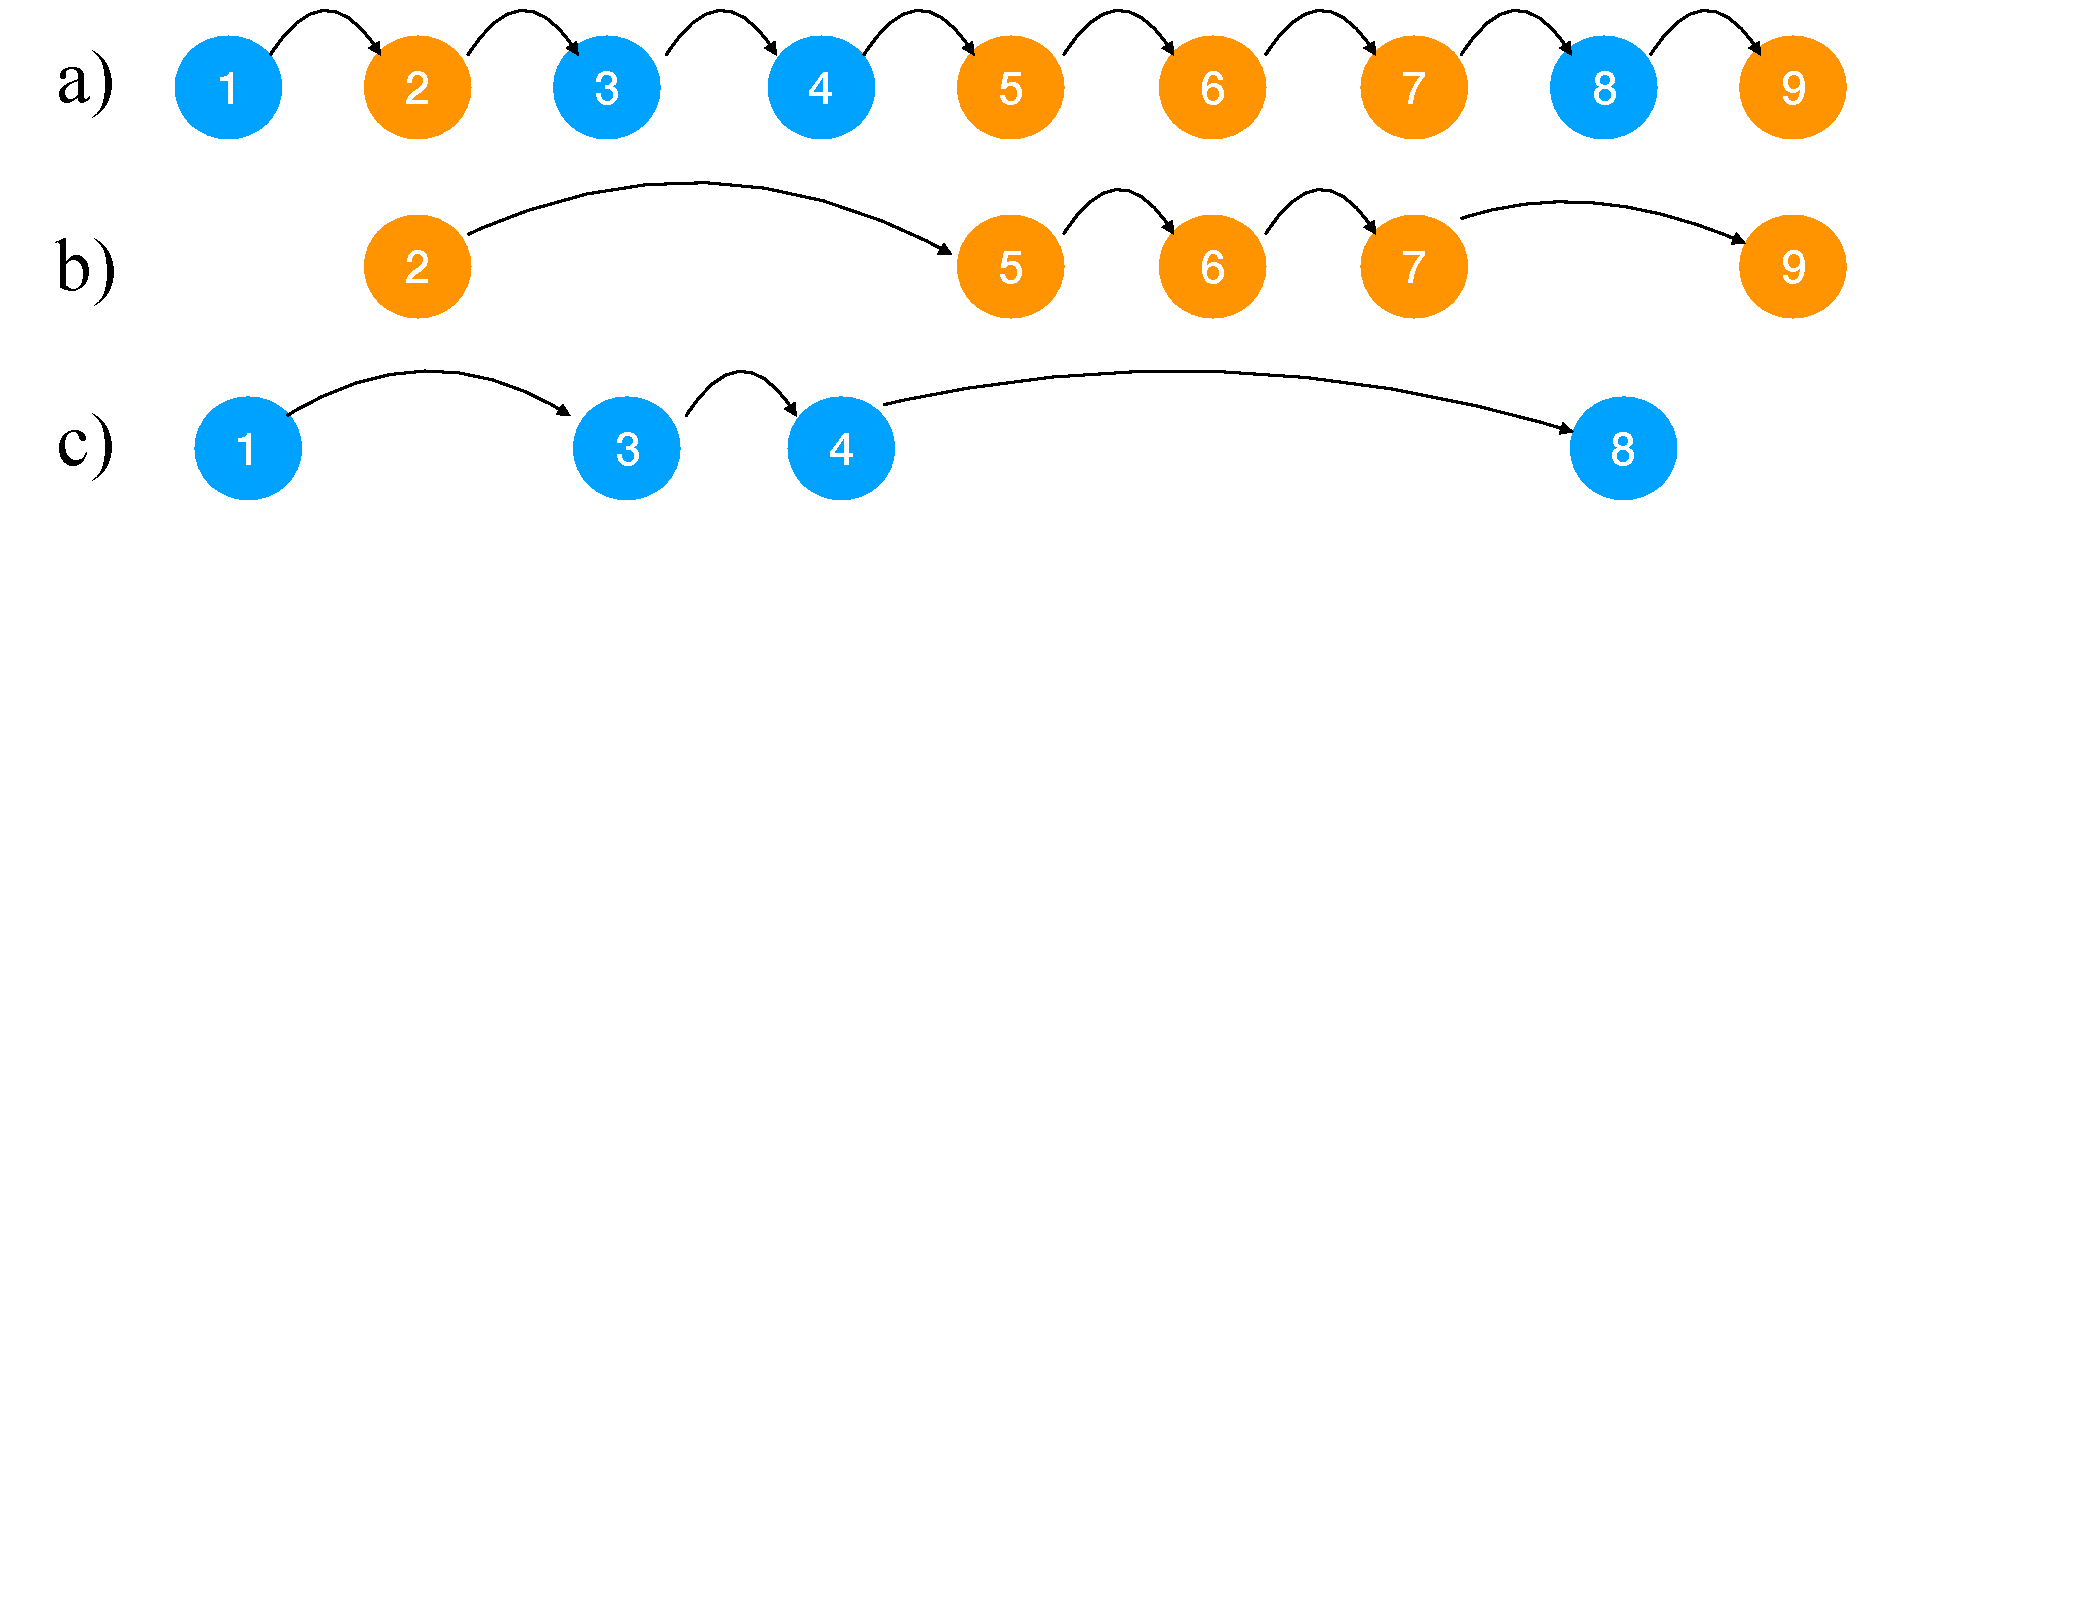
\includegraphics[width=\linewidth]{diagrams/VisibleStates.pdf}
     \end{center}
   \end{minipage}
   \end{center}
   \vspace*{-2.5mm}
   \caption{Two Module Execution
     (Def. \ref{def:execution:internal:external}). %
     %
     a) $\M_1 \link \M_2$ b) $\M_1 \mkpair \M_2$ c) $\M_2 \mkpair \M_1$}
   \label{fig:VisibleStates}
   \Description{Three rows of circles coloured blue and orange. In the top row are 9 circles labelled 1 through 9. Some are coloured blue, and some are coloured orange. In the next row, only the orange circles from the first are shown. In the final row, only the blue circles. Arrows connect successive circles in each row.}
 \end{figure}

Two-module execution  is related to % the concept of 
visible states
semantics \cite{MuellerPoetzsch-HeffterLeavens06} as they both filter configurations, with  the difference
that in visible states semantics % \sd{considers all intermediate configurations during execution, but
execution is unfiltered and  configurations are only filtered when it comes to the  consideration 
of class invariants while two-module execution filters execution.
%
The lemma below says  that linking is associative and commutative, and preserves   both one-module and two-module execution.

\begin{lemma}[Properties of linking]
\label{lemma:linking}
 For any modules $\M$,   $\M'$, $\M''$, and $\M'''$ and runtime configurations $\sigma$, and $\sigma'$ we have$:$
 \label{lemma:linking:properties}

 \begin{itemize}
     \item
     $(\M \link \M')\link \M''$ = $\M \link (\M' \link \M'')$  \hspace{1cm} and    \hspace{1cm}   $\M \link \M'$  = $\M' \link\M$.
      \item
      $\M, \sigma \leadsto \sigma'$, and $\M\link \M'$ is defined, \  \ \ \ \  implies\ \ \ \ \   $\M\link \M', \sigma \leadsto \sigma'$.
 \item
 $\M \mkpair \M', \sigma \leadsto \sigma'$   \  \ \ \ \  implies\ \ \ \ \  $(\M\link\M'') \mkpair (\M'\link\M''') ,\sigma \leadsto \sigma'$.  
  \end{itemize}

 \end{lemma}
 
 We can now answer the question as to which runtime configurations are pertinent when judging a module's
adherence to an assertion.
{\em Initial configurations} are those whose heap  have only one object, of class \prg{Object}, and whose stack have one frame, with arbitrary continuation.
{\em Arising} configurations are  those that can be reached by two-module execution, starting from a specific initial configuration to maintain temporal linearity.
 
\begin{definition}[Initial and Arising Configurations] defined as follows, using the semantics from Definition~\ref{def:runtimeentities}: \label{def:arise}

\begin{itemize}
     \item
   $\Initial {(\psi,\chi)}$, \ \ if \ \ $\psi$ consists of a single frame $\phi$ with $dom(\phi)=\{ \this \}$, and there exists  some address $\alpha$, such that \ \ \    $\interp {\this}{\phi}$=$\alpha$, and \ $dom(\chi)$=$\alpha$,\  and\  
    $\chi(\alpha)=(\prg{Object},\emptyset)$.
 \item
 $\Arising  {\M\mkpair\M', \sigma_0} \ = \ \{ \ \sigma \ \mid \ \Initial{\sigma_0}\ \wedge\ \M\mkpair\M', \sigma_0 \leadsto^* \sigma \ \ \} $
 \end{itemize}

\end{definition}
\jm{Arising configurations differ in their definition to that of previous work published at FASE 2020~\cite{FASE} in the usage of an initial configuration. In prior work
an arising configuration was defined as any configuration that might arise from {\em any} initial configuration. In linearizing Chainmail, we specify a specific initial 
configuration.}
